\chapter{Systemablaufmodell}\label{ch:systemablaufmodell}

Abbildung \ref{fig:systemablaufmodell} zeigt den Ablauf aller Geschäftsfälle.
Hierbei werden insbesondere die Beziehungen zwischen den einzelnen Geschäftsfällen und den beteiligten Systemen deutlich.
Etwaige Ausnahmen werden in den Diagrammen der einzelnen Geschäftsfällen berücksichtigt.

\begin{figure}[H]
    \centering
    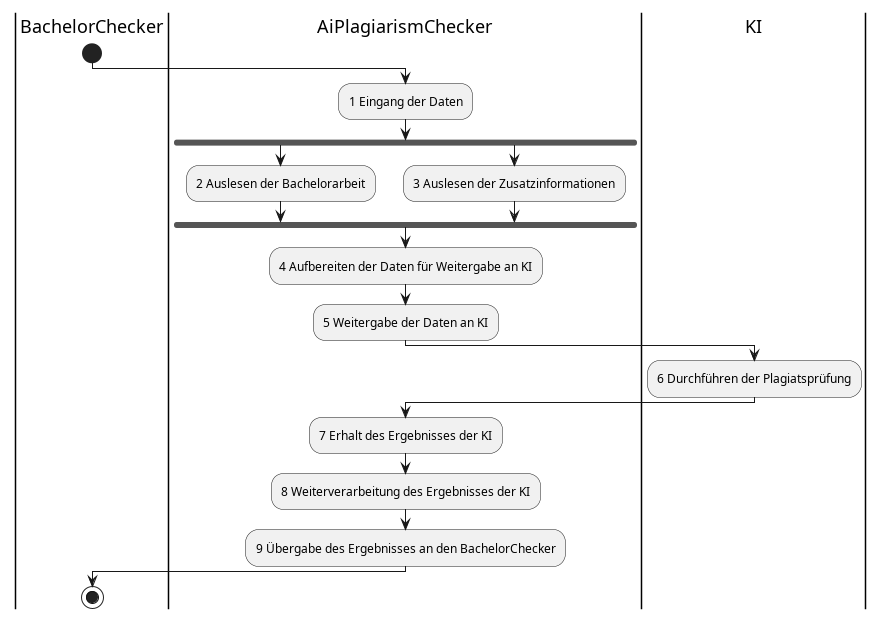
\includegraphics[width=1\textwidth]{out/diagrams/businessProcessDiagram/Systemablaufmodell.png}
    \caption{Systemablaufmodell}
    \label{fig:systemablaufmodell}
\end{figure}

\newpage Die nachfolgenden Diagramme zeigen die Systemabläufe der einzelnen Geschäftsfälle.
Der letzte Schritt in einem Geschäftsfall ist immer gleichzeitig die Benennung des Endknotens.

\begin{figure}[H]
    \centering
    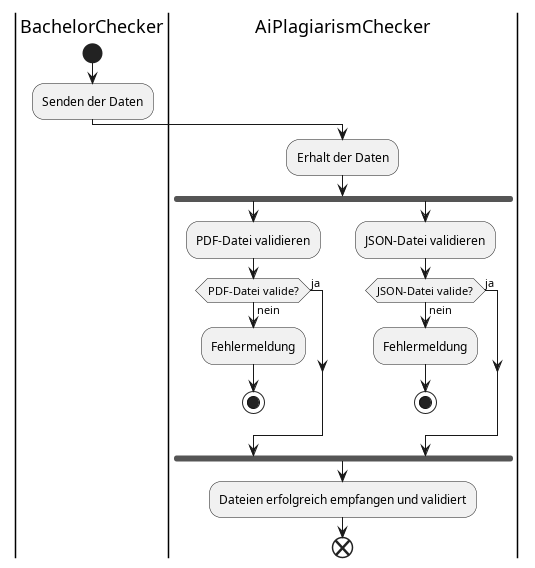
\includegraphics[width=0.9\textwidth]{out/diagrams/bpd/EingangDerDatenVomBachelorChecker/GPD-Eingang der Daten vom BachelorChecker.png}
    \caption{Eingang der Daten vom BachelorChecker}
    \label{fig:eingangDerDatenVomBachelorChecker}
\end{figure}

\begin{figure}[H]
    \centering
    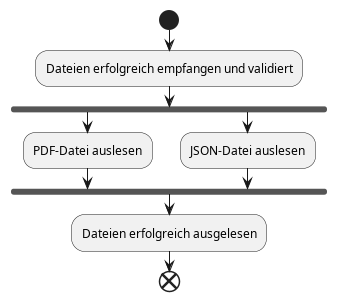
\includegraphics[width=0.55\textwidth]{out/diagrams/bpd/AuslesenDerBachelorarbeit/GPD-Auslesen der Bachelorarbeit.png}
    \caption{Auslesen der Bachelorarbeit und der Zusatzinformationen}
    \label{fig:auslesenDerBachelorarbeit}
\end{figure}

\begin{figure}[H]
    \centering
    \includegraphics[width=0.4\textwidth]{out/diagrams/bpd/AufbereitenDerDatenFuerWeitergabeAnKI/GPD-Aufbereiten der Daten für Weitergabe an KI.png}
    \caption{Aufbereiten der Daten für Weitergabe an KI}
    \label{fig:aufbereitenDerDatenFuerWeitergabeAnKI}
\end{figure}

\begin{figure}[H]
    \centering
    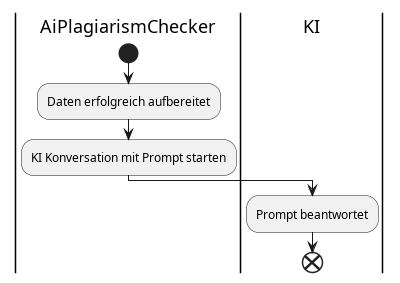
\includegraphics[width=0.65\textwidth]{out/diagrams/bpd/WeitergabeDerDatenAnKI/GPD-Weitergabe der Daten an KI.png}
    \caption{Weitergabe der Daten an KI}
    \label{fig:weitergabeDerDatenAnKI}
\end{figure}

\begin{figure}[H]
    \centering
    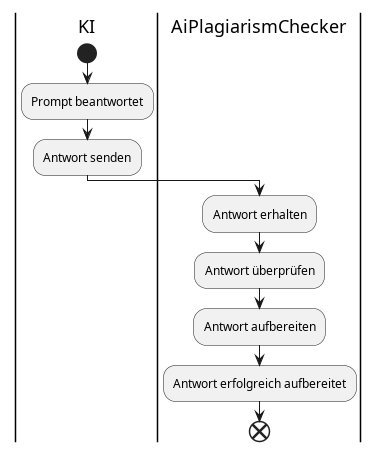
\includegraphics[width=0.6\textwidth]{out/diagrams/bpd/ErhaltDesErgebnissesDerKI/GPD-Erhalt des Ergebnisses der KI.png}
    \caption{Erhalt des Ergebnisses der KI}
    \label{fig:erhaltDesErgebnissesDerKI}
\end{figure}

\begin{figure}[H]
    \centering
    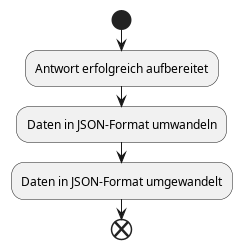
\includegraphics[width=0.4\textwidth]{out/diagrams/bpd/WeiterverarbeitungDesErgebnissesDerKI/GPD-Weiterverarbeitung des Ergebnisses der KI.png}
    \caption{Weiterverarbeitung des Ergebnisses der KI}
    \label{fig:weiterverarbeitungDesErgebnissesDerKI}
\end{figure}

\begin{figure}[H]
    \centering
    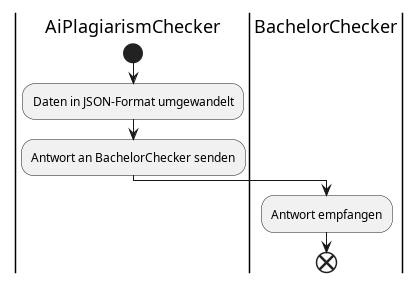
\includegraphics[width=0.65\textwidth]{out/diagrams/bpd/ÜbergabeDesErgebnissesAnDenBachelorChecker/GPD-Übergabe des Ergebnisses an den BachelorChecker.png}
    \caption{Übergabe des Ergebnisses an den BachelorChecker}
    \label{fig:uebergabeDesErgebnissesAnDenBachelorChecker}
\end{figure}

